\chapter{The Pythagorean Theorem}

\section{Try it first}
Before reading any proof, try a little experiment.

Draw a right triangle (a triangle with one square corner). Call the two short
sides \(a\) and \(b\), and call the longest side \(c\).

\begin{itemize}
  \item Try one triangle with \(a=3\), \(b=4\), and measure \(c\).
  \item Try another with \(a=5\), \(b=12\), and measure \(c\).
  \item Try your own triangle and measure all three sides.
\end{itemize}

Now compare \(a^2+b^2\) with \(c^2\). You will probably see they match.
That is exciting, but examples are not a proof.

\section{Why examples are not enough}
In mathematics, checking many examples is useful, but it cannot prove a rule
for \emph{every} case.

Here is a famous idea:
\begin{quote}
Seeing \(1000\) white swans, or even \(1\) million white swans, still does not
prove that \emph{all} swans are white.
\end{quote}

A proof must explain why the statement is always true, not only true in many
cases.

\section{A picture of \(a\), \(b\), and \(c\)}
Before proving anything, let us draw one right triangle and label the sides.

\begin{center}
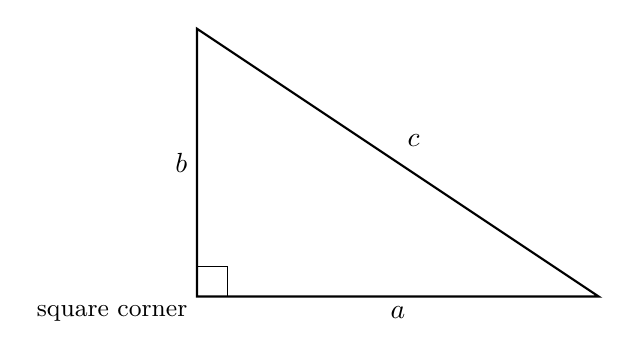
\begin{tikzpicture}[scale=0.85]
  % Triangle vertices
  \coordinate (A) at (0,0);
  \coordinate (B) at (6,0);
  \coordinate (C) at (0,4);

  % Triangle edges
  \draw[thick] (A) -- (B) -- (C) -- cycle;

  % Right-angle mark at A
  \draw (0,0) ++(0.45,0) -- ++(0,0.45) -- ++(-0.45,0);

  % Labels for sides
  \node[below] at (3,0) {\(a\)};
  \node[left] at (0,2) {\(b\)};
  \node[above right] at (3,2.1) {\(c\)};

  % Optional corner labels
  \node[below left] at (A) {\small square corner};
\end{tikzpicture}
\end{center}

\noindent
In this chapter, \(a\) and \(b\) are the two shorter sides that meet at the
square corner, and \(c\) is the longest side across from that corner.

\begin{center}
\begin{tabular}{|c|c|c|c|}
\hline
Example & \(a\) & \(b\) & \(c\) (measured) \\
\hline
1 & 3 & 4 & 5 \\
\hline
2 & 5 & 12 & 13 \\
\hline
3 & 8 & 15 & 17 \\
\hline
4 & 7 & 24 & 25 \\
\hline
\end{tabular}
\end{center}

\noindent
These examples show a pattern, but a pattern is still not a proof.

\section{How to find a proof}
Think of proof-search like route-search.

You start in one place (your question) and want to reach another place (a
statement that must be true). Between them are many possible roads (ideas,
drawings, identities, and known facts). Finding a proof means finding a
connected path that really reaches the destination.

For example, imagine traveling from a small city in Germany to a small town in
Malaysia. You would not jump directly in one step. You might go:
\[
\text{small city} \rightarrow \text{nearby rail hub} \rightarrow \text{major airport}
\rightarrow \text{Kuala Lumpur} \rightarrow \text{small town}.
\]
At each step, you ask: ``Can I really go from here to there?'' If yes, keep
moving. If no, choose another route.

Proof works the same way. For the Pythagorean theorem, our start is
``many triangles seem to follow a pattern.'' Our destination is
``this is always true for every right triangle.'' In the next section, we will
choose good intermediate stops and build a complete path.

\section{First Proof: Rearrangement by Drawing}
There are many ways to prove the Pythagorean theorem (for example, geometric
rearrangement, similar triangles, and Euclid-style area arguments). Here we
start with a rearrangement picture approach.

Our target is simple:
\begin{quote}
We are finding the values of \(a^2\), \(b^2\), and summing them. Once we can
show that this sum is the same as \(c^2\), we are done.
\end{quote}

\noindent
The drawing below shows two big squares, each with side \(a+b\). Inside each
big square we place four identical right triangles (legs \(a,b\), hypotenuse
\(c\)) in different ways.

\begin{center}
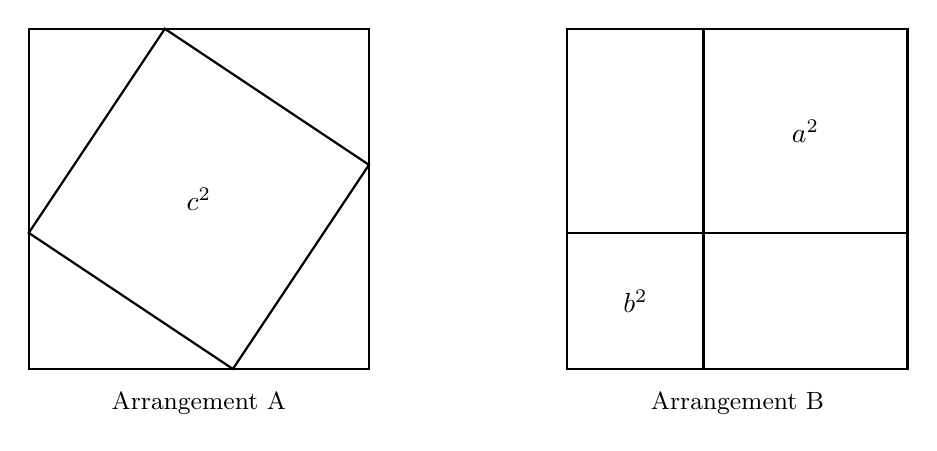
\begin{tikzpicture}[scale=0.72]
  % ---------- Left big square ----------
  \draw[thick] (0,0) rectangle (6,6);
  % center c^2 square (diamond style)
  \draw[thick] (0,2.4) -- (2.4,6) -- (6,3.6) -- (3.6,0) -- cycle;
  \node at (3,3) {\(c^2\)};
  \node at (3,-0.6) {\small Arrangement A};

  % ---------- Right big square ----------
  \begin{scope}[xshift=9.5cm]
    \draw[thick] (0,0) rectangle (6,6);
    % inner split showing a^2 and b^2 blocks
    \draw[thick] (2.4,2.4) rectangle (6,6);
    \draw[thick] (0,0) rectangle (2.4,2.4);
    \node at (4.2,4.2) {\(a^2\)};
    \node at (1.2,1.2) {\(b^2\)};
    \node at (3,-0.6) {\small Arrangement B};
  \end{scope}
\end{tikzpicture}
\end{center}

\noindent
Why this works: both big squares have the same outside area \((a+b)^2\), and
both use the same four triangles. So the leftover middle area must also be the
same in both pictures. In Arrangement A, the leftover is \(c^2\). In
Arrangement B, the leftover is \(a^2+b^2\). Therefore the leftovers match:
\[
a^2+b^2=c^2.
\]

